\documentclass{standalone}
\usepackage{tikz}
\usetikzlibrary{decorations.pathmorphing, calc}
\usetikzlibrary{patterns}

\begin{document}

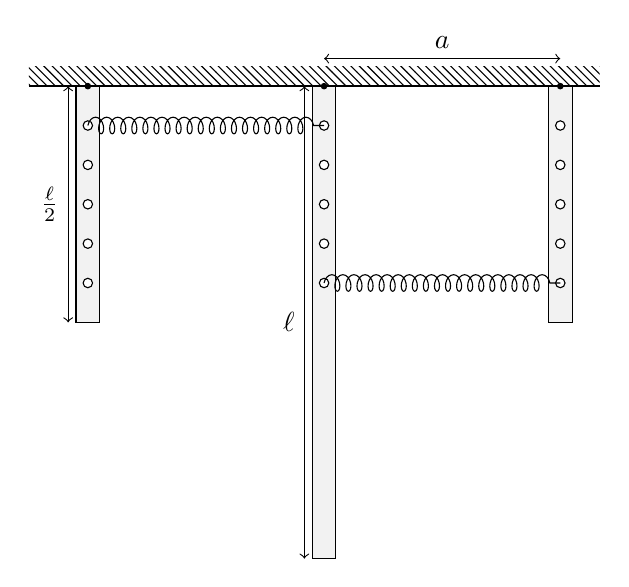
\begin{tikzpicture}
	% Parameters
	\def\pivoty{0}
	\def\pivotsep{3}
	\def\length{3}
	\def\lengthtwo{6} % Different length for middle pendulum
	\def\rodwidth{0.3}
	\def\holecount{5}
	\def\holeradius{0.06}
	\def\tol{0.01}

	% Light auxiliary grid (comment to remove)
	% \draw[step=0.5cm, gray!20, very thin] (-2,-5) grid (8,1);

	% Ceiling
	\fill[pattern=north west lines] (-0.75, \pivoty) rectangle (2*\pivotsep+0.5, \pivoty+0.25);
	\draw[thick] (-0.75, \pivoty) -- (2*\pivotsep+0.5, \pivoty);

	% Pivots
	\coordinate (P1) at (0, \pivoty);
	\coordinate (P2) at (\pivotsep, \pivoty);
	\coordinate (P3) at (2*\pivotsep, \pivoty);

	% End positions (straight down)
	\coordinate (M1) at ($(P1) + (270:\length)$);
	\coordinate (M2) at ($(P2) + (270:\lengthtwo)$);
	\coordinate (M3) at ($(P3) + (270:\length)$);

	% Compute hole heights from first pendulum
	\foreach \j in {1,...,\holecount} {
		\pgfmathsetmacro\relpos{\j/(\holecount+1)}
		\path let \p1 = (P1), \p2 = (M1) in
			coordinate (H\j) at ($(\p1)!\relpos!(\p2)$);
	}

	% Rods
	\foreach \i/\P/\M/\L in {1/P1/M1/\length, 2/P2/M2/\lengthtwo, 3/P3/M3/\length} {
		\path (\P) -- (\M) coordinate[pos=0] (Top\i);
		\path (\P) -- (\M) coordinate[pos=1] (Bottom\i);

		\path let \p1 = (Top\i), \p2 = (Bottom\i) in
			coordinate (TopLeft\i) at ($(\p1)+(-\rodwidth/2,0)$)
			coordinate (TopRight\i) at ($(\p1)+(\rodwidth/2,0)$)
			coordinate (BottomRight\i) at ($(\p2)+(\rodwidth/2,0)$)
			coordinate (BottomLeft\i) at ($(\p2)+(-\rodwidth/2,0)$);
		\draw[fill=gray!10] (TopLeft\i) -- (TopRight\i) -- (BottomRight\i) -- (BottomLeft\i) -- cycle;

		% Coupling holes
		\foreach \j in {1,...,\holecount} {
			\path (P1 |- H\j) coordinate (HoleRef);
			\path let \p1 = (HoleRef), \p2 = (\M) in
				coordinate (Temp) at (\P |- H\j);
			\fill[white] (\P |- H\j) circle (\holeradius);
			\draw[black] (\P |- H\j) circle (\holeradius);
		}
	}

	% Pivot holes
	\foreach \i in {1,2,3}
	\fill[black] (P\i) circle (1.2pt);

	% Labels Length
	\draw[<->] ($(M1)-(0.25,0)$) -- node[left] {$\frac{\ell}{2}$} ($(P1)-(0.25,0)$);
	\draw[<->] ($(M2)-(0.25,0)$) -- node[left] {$\ell$} ($(P2)+(-.25,0)$);
	% Label horizontal
	\draw[<->] ($(P2)+(0.0,0.35)$) -- node[above] {$a$} ($(P3)+(0.0,0.35)$);

	% Springs between masses
	% Spring from hole 1 of M1 and M2
	\coordinate (S12a) at (P1 |- H1);
	\coordinate (S12b) at (P2 |- H1);
	\draw[decorate, decoration={coil, aspect=0.6, segment length=4pt, amplitude=3pt}]
		(S12a) -- (S12b);

	% Spring from hole 5 of M2 and M3
	\coordinate (S23a) at (P2 |- H5);
	\coordinate (S23b) at (P3 |- H5);
	\draw[decorate, decoration={coil, aspect=0.6, segment length=4pt, amplitude=3pt}]
		(S23a) -- (S23b);

\end{tikzpicture}

\end{document}

